\documentclass[xcolor={dvipsnames}, 11pt]{beamer}
\usetheme{Warsaw}


\setbeamercolor*{palette primary}{use=structure,fg=Blue,bg=CornflowerBlue!70!MidnightBlue}
\setbeamercolor*{palette quaternary}{fg=CornflowerBlue,bg=MidnightBlue}
\setbeamercolor*{item}{fg=MidnightBlue}
\setbeamertemplate{navigation symbols}{}
\setbeamertemplate{caption}[numbered]

\usepackage[serbian]{babel} 
\usepackage[utf8]{inputenc} 
\usepackage{amsmath}
\usepackage{amsfonts}
\usepackage{amssymb}
\usepackage{graphicx}
\usepackage{multicol}

\author{Ajzenhamer Nikola \\ Bukurov Anja \\ Stankovi\' c Vojislav }
\title{Sinergija}

%\logo{
\includegraphics[height=1.8cm]{logo.png}\vspace{220pt}}

%institute{}

%date{}

%subject{}

%setbeamercovered{transparent}

%setbeamertemplate{navigation symbols}{}

\begin{document}
%	\maketitle

\begin{frame}
	\titlepage
\end{frame}

\section{Sinergija}

\begin{frame}{Opis}
Sinergija je veb aplikacija \v cija je namena ubrzanje i pobolj\v sanje pra\' cenja rada u Studentskoj organizaciji Matemati\v ckog fakulteta OMIKRON (u daljem tekstu: OMIKRON). Omogu\' cava \v clanovima OMIKRON-a da na jednostavan na\v cin upravljaju svojim obavezama, kao i da ih pregledaju, \v cime se \v citava komunikacija me\dj u \v clanovima svodi na jedno mesto.
\end{frame}
		
\begin{frame}{Ciljevi}
	\begin{enumerate}

		\item Ubrzanje i pobolj\v sanje rada u OMIKRON-u.
		\item Upravljanje obavezama iz centralizovanog sistema.
		\item Svo\dj enje komunikacije me\dj u \v clanovima na jednu platformu.
		

	\end{enumerate}
\end{frame}
	
\section{Tehni\v cki detalji}

\subsection{Kori\v s\' cene tehnologije}

\begin{frame}{Kori\v s\' cene tehnologije}
	\begin{itemize}
		\item Back-end:
		\begin{itemize}
			\item PHP
			\item MySQL
		\end{itemize}
		
		\item Front-end:
		\begin{itemize}
			\item JavaScript
			\item jQuery
		\end{itemize}
		
		\item Dizajn stranica:
		\begin{itemize}
			\item Twig
			\item Foundation
		\end{itemize}
	\end{itemize}
	
\end{frame}

\subsection{Shema baze}

\begin{frame}{Tabele}
	\begin{multicols}{2}
		\begin{itemize}
			\item Korisnik
			\item Obaveza
			\item Ima obavezu
			\item Projekat
			\item Tim
			\item U\v cestvuje
			\item Koordinira
			\item Prijatelji
			\item Zadu\v zen
			\item Log
			\item Privatna poruka
		\end{itemize}
	\end{multicols}	
\end{frame}

\begin{frame}
	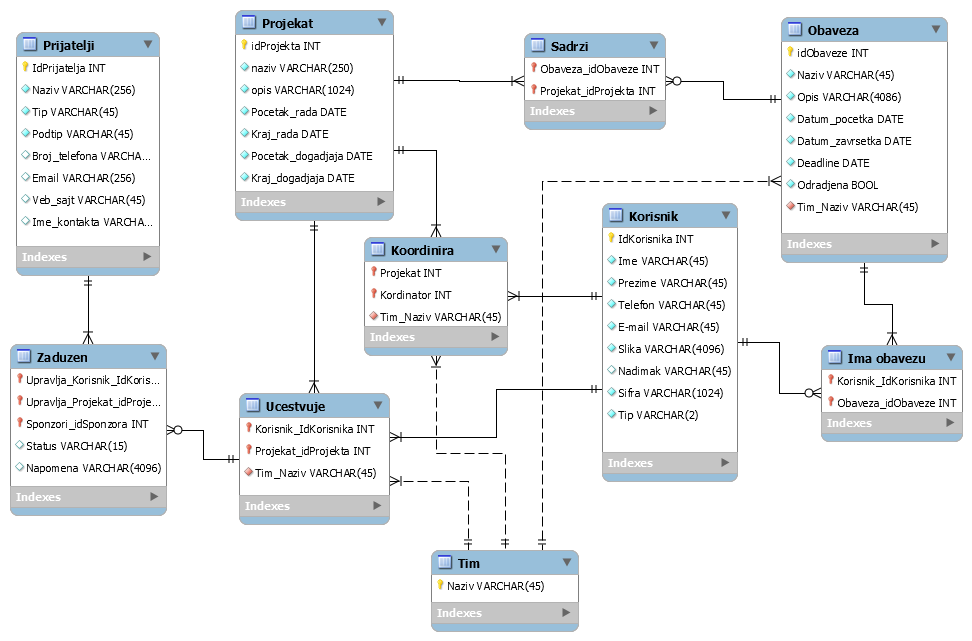
\includegraphics[width=\linewidth]{shema.png}
\end{frame}

\section{Razvijene mogu\' cnosti}

\subsection{\v Clanovi organizacije}
\begin{frame}{\v Clanovi organizacije}
	\begin{itemize}
		\item Pristupanje sistemu
		\item Izmena podataka o \v clanu
		\item Izmena profilne slike
		\item Sistem privatnih poruka
		\item Sistem sobe za \' caskanje
		\item Pregledanje obaveza i zadu\v zenja kontaktiranja prijatelja
		\item Podnos izve\v staja kontaktiranja prijatelja
	\end{itemize}
\end{frame}

\subsection{\v Clanovi upravnog odbora}
\begin{frame}{\v Clanovi upravnog odbora}
	\begin{itemize}
		\item Kreiranje novih i brisanje postoje\' cih \v clanova
		\item Kreiranje novih obaveza
		\item Kreiranje novih projekata
		\item Odre\dj ivanje koordinatora prijekta za svaki tim
		\item Dodavanje prijatelja organizacije i izmena njihovih podataka
		\item Delegiranje zadu\v zenja kontaktiranja prijatelja
	\end{itemize}
\end{frame}

\subsection{Koordinatori projekta}
\begin{frame}{Koordinatori projekta}
	\begin{itemize}
		\item Kreiranje novih obaveza na projektu
		\item Delegiranje zadu\v zenja kontaktiranja prijatelja na projektu
	\end{itemize}
\end{frame}

\section{Pitanja}
\begin{frame}
	Pitanja?
\end{frame}

\begin{frame}
	Hvala na pa\v znji!
\end{frame}
	
	
\end{document}